\section{Vzorkovací obvody}
- S/H a T/H obvody - rozdíly, funkce, základní parametry, příklady realizací
\subsection{S/H a T/H obvody}
\textbf{Vzorkovač s pamětí – S/H (sample and hold)}, který sejme v daném okamžiku vzorek signálu a podrží si jeho hodnotu, při příchodu dalšího řídicího pulzu uloží novou, aktuální hodnotu.

\textbf{Sledovač s pamětí – T/H (track and hold)}, sleduje (kopíruje) průběh signálu a ukládá si aktuální hodnotu až s příchodem řídicího impulzu.

\subsection{Funkce}
Vzorkovače plní důležitou funkci v rámci převodníku. Spojitý signál (spojitý v čase i hodnotě) na vstupu vzorkují a na výstupu poskytují spojitý signál, ale diskrétní v hodnotě. Tento signál je zpracováván pomocí kvantovacího obvodu, který příslušné diskrétní hodnotě (hladině) přidělí odpovídající binární hodnotu s maximální chybou ½ LSB.
\subsection{Základní parametry}
\textbf{Zesílení (gain)} je střední strmost statické převodní charakteristiky. Udává se možná
chyba zesílení a rozsah seřizovacích možností.

\textbf{Vstupní napěťový rozsah (input voltage range)} je povolené napětí, při kterém platí
jmenovité parametry.

\textbf{Výstupní napěťový rozsah (output voltage range)} je rozsah výstupního napětí, kdy ještě
nedochází k omezení výstupního napětí.

\textbf{Vstupní napěťová nesymetrie (input voltage offset)} je vstupní napětí, při kterém je
výstupní právě rovno nule

\textbf{Nelinearita (linearity)} udává maximální odchylku výstupního napětí od jmenovité hodnoty. Měří se po přesném nastavení zesílení a vynulování offsetu, udává se většinou v \%.

\textbf{Činitel potlačení vstupního napětí (feedthrough rejection ratio)} udává převrácenou
hodnotu přenosu vstupního napětí na výstup v paměťovém provozu. Někdy se udává
v závislosti na kapacitě paměťového kapacitoru. Jednotkou obvykle bývá dB.

\textbf{Rychlost klesání výstupního napětí (droop rate)} je změna výstupního napětí za jednotku
času po zapamatování napětí. Je způsobeno svodovými proudy paměťového kapacitoru a
klidovými proudy připojených obvodů. Obvykle se udává v závislosti na kapacitě
paměťového kapacitoru.
   \begin{figure}[h]
   \begin{center}
     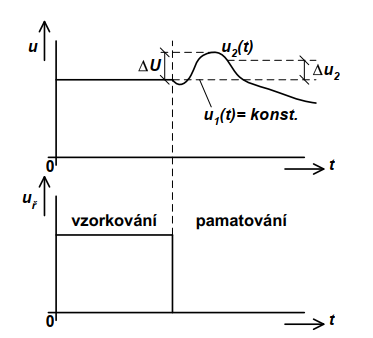
\includegraphics[scale=0.6]{images/Droop.png}
   \end{center}
   \caption{Skutečný průběh pamatování ve vzorkovači}
  \end{figure}
\pagebreak

\subsubsection{Základní parametry související s přechodovými ději}
\textbf{Doba upnutí (acquisition time)} je doba potřebná k přechodu z paměťového do sledovacího provozu. Definuje se pro udaný skok výstupního napětí (nejhorší je skok přes celé rozmezí povoleného výstupního napětí) s následným ustálením v předepsaném tolerančním pásu při ss nebo pomalu se měnícím vstupním napětí

\textbf{Rychlost přeběhu (slew rate)} je maximální rychlost změny výstupního napětí. U provedení s vnějším C\textsubscript{p} se udává v závislosti na tomto kapacitoru nebo se udává maximální nabíjecí proud I\textsubscript{max} (buď konečný proud, který je schopen dodat předřazený OZ nebo proud, který může téct maximálně spínačem – volí se ten, který je menší). Uvažují-li se neomezené proudové schopnosti zdroje vstupního signálu, pak se při vzorkování C\textsubscript{p} nabíjí přes sériovou kombinaci nenulového vnitřního odporu zdroje vstupního signálu R\textsubscript{i} a odporu sepnutého spínače R\textsubscript{sep} s časovou konstantou:
\begin{equation}
\tau = (R_{i}+R_{sep}*C_{p})
\end{equation}

Doba vzorkování nutná pro dosažení dané přesnosti
\begin{itemize}
\item pro přesnost 10\%: 
\begin{equation}
\tau \geq 3*(R_{i}+R_{sep}*C_{p})
\end{equation}
\item pro přesnost 1\%: 
\begin{equation}
\tau \geq 5*(R_{i}+R_{sep}*C_{p})
\end{equation}
\item pro přesnost 0,1\%: 
\begin{equation}
\tau \geq 7*(R_{i}+R_{sep}*C_{p})
\end{equation}
\item pro přesnost 0,01\%: 
\begin{equation}
\tau \geq 9*(R_{i}+R_{sep}*C_{p})
\end{equation}
\end{itemize}

\textbf{Doba ustálení (settling time)} je doba potřebná k přechodu ze vzorkovacího do ustáleného paměťového režimu. Měří se doba ustálení signálu v daném tolerančním pásmu.

\textbf{Přepínací skokové napětí (sample-to-hold offset)} je chyba sejmutí vzorku v důsledku
průniku řidicího signálu přes parazitní kapacity spínače. V provedení s vnějším C\textsubscript{p} se uvede
velikost náboje přeneseného na C\textsubscript{p}.

\textbf{Apertura (časová neurčitost – aperture)} je způsobena reálnými vlastnostmi těch částí
vzorkovače, které realizují přechod obvodu z režimu vzorkování do pamatování.

\textbf{Efektivní okamžik sejmutí vzorku (effective sampling time) t\textsubscript{ef}} je okamžik, v němž by
měl monotónně se měnící vstupní signál velikost, na které se ustálí napětí na C\textsubscript{p}.

\textbf{Doba apertury (aperture time)} je doba mezi bezprostředním pokynem k rozpojení
spínače a ukončením rozpojování, kdy lze spínač považovat za zcela rozpojený.

\textbf{Nejistota apertury (aperture uncertainty)} je náhodné kolísání doby apertury. Někdy se
označuje jako aperturové chvění (jitter).

\textbf{Fázové zpoždění (phase delay)} je doba mezi bezprostředním podnětem k rozpojení
spínače a \textsubscript{ef}.

\textbf{Aperturová chyba (aperture error)} je nepřesnost sejmutí vzorku v důsledku aperturového
chvění a s kmitočtem roste
   \begin{figure}[h]
   \begin{center}
     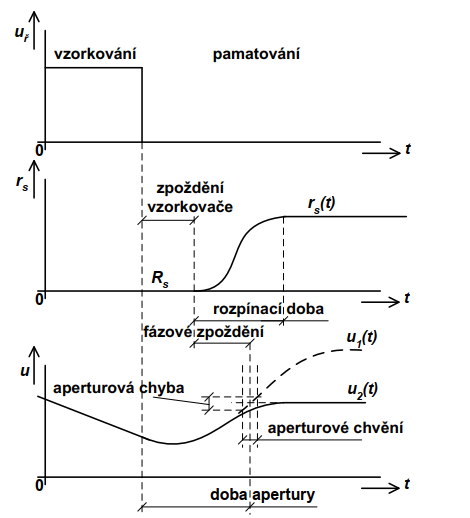
\includegraphics[scale=0.6]{images/Apertura.png}
   \end{center}
   \caption{Apertura}
  \end{figure}
  
\textbf{Zpoždění vzorkovače (S/H delay, T/H delay)} je doba mezi příkazem k sejmutí vzorku a bezprostředním podnětem k rozpojení spínače.

\subsection{Příklady realizací}
Realizace vzorkovače je v drtivé většině případů řešena zapojením v technice SC. V současné době se však dostává do popředí zájmu i technika spínaných proudů (SI) a to zejména díky pracovnímu režimu, který je proudový, čehož je využíváno ke snižování napájecích napětí.

\subsubsection{Neinvertující zapojení vzorkovačů s pamětí v technice SC}
Při sepnutém spínači S je paměťový kapacitor C\textsubscript{p} připojen ke zdroji snímaného napětí. Po dobu sepnutí TS se kapacitor 
C\textsubscript{p} nabíjí na napětí odpovídající skutečné hodnotě vstupního signálu. Současně se odpovídajícím způsobem mění výstupní napětí oddělovacího zesilovače, kterým je většinou OZ v neinvertujícím zapojení. Po rozpojení spínače S se na kapacitoru 
C\textsubscript{p} a tedy i na výstupu
zesilovače udržuje napětí sejmutého vzorku. Doba T\textsubscript{S} odběru vzorku je velmi krátká a je proto použit elektronický spínač. Protože však u těchto spínačů nejsou splněny podmínky pro ideální spínače, tj. R\textsubscript{ON} = 0, R\textsubscript{OFF} -> $\infty$, nabíjí se paměťový kapacitor exponenciálně s časovou konstantou:
\begin{equation}
\tau = R_{s}*C_{p}
\end{equation}
,kde
\begin{equation}
R_{s} = R_{ON}+ R_{i}
\end{equation}
R\textsubscript{ON} je odpor sepnutého spínače a odpor R\textsubscript{i} zdroje vstupního signálu.
\begin{figure}[h]
   \begin{center}
     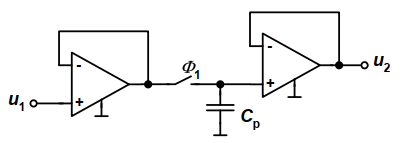
\includegraphics[scale=0.6]{images/VzorSC.png}
   \end{center}
   \caption{Základní neinvertující zapojení vzorkovače}
\end{figure}

Dynamické vlastnosti lze zlepšit volbou vhodných rychlých součástek (velmi rychlé OZ, rychlý převodník napěťových úrovní pro vlastní spínač, realizace spínače diodovým můstkem se Schottkyho diodami, volbou malé kapacity paměťového kapacitoru, značným proudovým dimenzováním výstupu prvního OZ).

Velké zesílení prvního OZ způsobuje, že se Cp nabíjí z většího napětí a to po dobu, dokud napětí na diferenčních vstupech prvního OZ nebudou stejná. Nevýhodou je přechod zmíněného OZ do saturace při rozpojení spínače

Aby se dosáhlo zvětšení nabíjecí rychlosti při změnách vstupního napětí o celý rozsah, připojí se paralelně k paměťovému kapacitoru spínač, který ho těsně před vlastním vzorkováním vybije. Nevýhodou je trochu složitější řídicí logika:

\begin{figure}[h]
   \begin{center}
     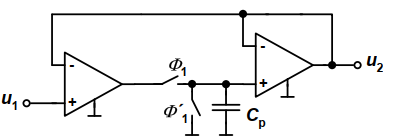
\includegraphics[scale=0.6]{images/VzorSC2.png}
   \end{center}
   \caption{Zapojení pro zvýšení nabíjecí rychlosti}
\end{figure}
\pagebreak  
Další úpravou, aby se zabránilo saturaci prvního OZ, je přidání zpětnovazebního odporu a spínač ve zpětnovazební smyčce bývá také velmi často nahrazen antiparalelním zapojením dvojice diod. 
\begin{figure}[h]
   \begin{center}
     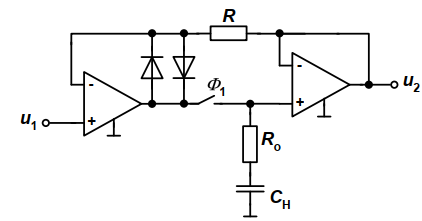
\includegraphics[scale=0.6]{images/VzorSC3.png}
   \end{center}
   \caption{Zapojení s dvojicí diod a opatřením proti saturaci}
\end{figure}
  
\subsubsection{Invertující zapojení vzorkovače v technice SC}
V případě invertujícího zapojení vzorkovače bývá paměťový kapacitor zapojen ve zpětné vazbě OZ – tzv. Millerův integrátor. Potřebný nabíjecí proud dodá zesilovač (nikoliv tedy zdroj vstupního napětí), čímž jsou menší nároky na spínač, protože se pracuje do virtuální země OZ.
\begin{figure}[h]
   \begin{center}
     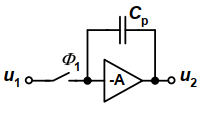
\includegraphics[scale=0.6]{images/Miller.png}
   \end{center}
   \caption{Základní zapojení Millerova integrátoru}
\end{figure} 
\newpage
\begin{figure}[t]
   \begin{center}
     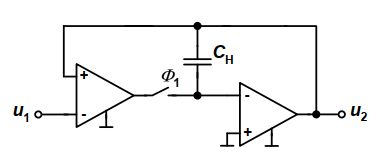
\includegraphics[scale=0.6]{images/VzorSC4.png}
   \end{center}
   \caption{Zlepšení vlastností základního invertujícího zapojení vzorkovače}
\end{figure}
Aby byla zajištěna záporná zpětná vazba v režimu vzorkování (spínač je sepnut), jsou
vstupní svorky prvního OZ zaměněny.
\begin{figure}[h]
   \begin{center}
     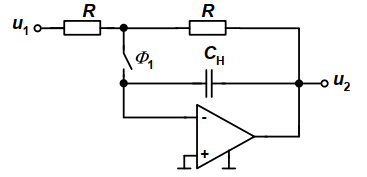
\includegraphics[scale=0.6]{images/VzorSC5.png}
   \end{center}
   \caption{Řešení invertujícího zapojení vzorkovače s volbou časové konstanty}
\end{figure}

Při sepnutí spínače bude paměťový kapacitor nabíjen s časovou konstantou:
\begin{equation}
\tau = (R_{s}+R)*C_{p}
\end{equation}
,kde R\textsubscript{S} je vnitřní odpor spínače. Proto je nutné volit R co nejmenší.


\begin{figure}[h]
   \begin{center}
     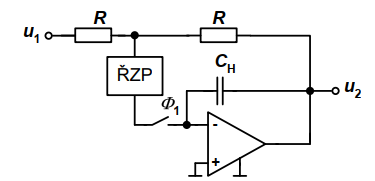
\includegraphics[scale=0.6]{images/VzorRZP.png}
   \end{center}
   \caption{Zkrácení doby nabíjení pomocí ŘZP}
\end{figure}
Velikost k\textsubscript{i} je omezena tím, že maximální hodnota nabíjecího proudu nemůže být větší než maximální výstupní proud OZ. Paměťový kapacitor musí být vybrán tak, aby měl malý svodový proud a malou dielektrickou absorpci.

\subsubsection{Vzorkovače v technice SI}
Paměťová buňka je základním prvkem v obvodech se spínanými proudy. Pro její funkci je využita parazitní kapacita CGS mezi hradlem a emitorem. Pro popsání základní funkce paměťové buňky je vhodné považovat tranzistor za ideální, tzn., že jsou zanedbány veškeré parazitní prvky kromě zmíněného kapacitoru C\textsubscript{GS}.
\begin{figure}[h]
   \begin{center}
     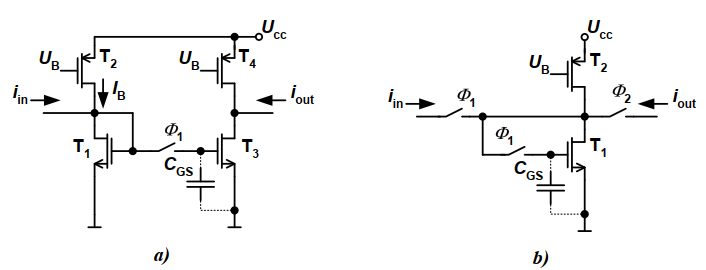
\includegraphics[scale=0.8]{images/VzorSI.png}
   \end{center}
   \caption{Vzorkovací obvody v technice SI a) buňka první generace b) buňka druhé generace}
\end{figure}










